\documentclass[12pt]{article}

\usepackage{float}

\usepackage{standalone}

\usepackage[utf8x]{inputenc}

%%% PAGE DIMENSIONS
\usepackage{geometry}
\geometry{a4paper}
\geometry{margin=2.54cm} % for example, change the margins to 2 inches all round

\usepackage{graphicx} % support the \includegraphics command and options

\usepackage[parfill]{parskip} % Activate to begin paragraphs with an empty line rather than an indent

%%% PACKAGES
\usepackage{booktabs} % for much better looking tables
\usepackage{array} % for better arrays (eg matrices) in maths
\usepackage{paralist} % very flexible & customisable lists (eg. enumerate/itemize, etc.)
\usepackage{verbatim} % adds environment for commenting out blocks of text & for better verbatim
\usepackage{subfig} % make it possible to include more than one captioned figure/table in a single float
% These packages are all incorporated in the memoir class to one degree or another...

\usepackage{multicol}
\usepackage{multirow}
\usepackage{xcolor}
\usepackage{amsmath}

\usepackage[T1]{fontenc}
\usepackage{lmodern}

% Sans-serif font
\renewcommand{\familydefault}{\sfdefault}

\usepackage{makecell}

\renewcommand{\arraystretch}{1.1}

%%% HEADERS & FOOTERS
\usepackage{fancyhdr} % This should be set AFTER setting up the page geometry
\pagestyle{fancy} % options: empty , plain , fancy
\fancyhead[L]{\leftmark}
\fancyhead[C]{}
\fancyhead[R]{\rightmark}
\fancyfoot[L]{}
\fancyfoot[C]{}
\fancyfoot[R]{\thepage}
\renewcommand{\headrulewidth}{0pt}
\renewcommand{\footrulewidth}{0pt}
\setlength{\headheight}{52pt}

\fancypagestyle{plain}{
	\fancyhf{} % clear all header and footer fields
	\fancyfoot[R]{\thepage} % except the center
	\renewcommand{\headrulewidth}{0pt}
	\renewcommand{\footrulewidth}{0pt}
}

%%% BIBILIOGRAPHY
\usepackage[numbers]{natbib}
\bibliographystyle{vancouver}

%%% SECTION TITLE APPEARANCE
\usepackage{sectsty}
\allsectionsfont{\sffamily\mdseries\upshape} % (See the fntguide.pdf for font help)
% (This matches ConTeXt defaults)

%%% ToC (table of contents) APPEARANCE
%\usepackage[nottoc,notlof,notlot]{tocbibind} % Put the bibliography in the ToC
%\usepackage[titles,subfigure]{tocloft} % Alter the style of the Table of Contents
%\renewcommand{\cftsecfont}{\rmfamily\mdseries\upshape}
%\renewcommand{\cftsecpagefont}{\rmfamily\mdseries\upshape} % No bold!

\usepackage[bookmarks,bookmarksnumbered,bookmarksopen,hidelinks]{hyperref}

\usepackage{bookmark}


%%% TITLE
\title{Statistical modelling of antibody data}
\author{Arseniy Khvorov, David J. Price, Annette Fox, Sheena G. Sullivan}
\begin{document}

%%% Title
\maketitle

%%% Main Contents

%==============================================================================
\section{Introduction}

In the study of infectious diseases it is useful to have some measure of whether a person is infected, immune or susceptible to infection. This may be important, for example, to understand disease prevalence, population-level susceptibility or for evaluation of vaccines.  However, direct measurement of immunity is often not possible and instead some \textit{correlate} of protection is used. For viral infectious diseases, an oft-used correlate is the serum antibody titre, which provides a measure of the amount of antibody that recognizes a particular epitope. 

Antibody titres have several limitations. Titres are the inverse of the greatest dilution of antibody that inhibits virus in serial dilutions, with higher values indicating greater inhibition. There is no true zero value, nor is there a true measure of the maximum value; titres can only be as low as the minimum starting concentration and as high as the maximum dilution.  Furthermore, within dilution intervals, the true concentration that inhibits virus is unknown; only the upper and lower bound of each dilution is known, i.e. titres are interval-censored. In addition, antibody titres are merely a surrogate measure and their sensitivity and specificity may be imperfect, such that reduced titres may not always correspond to increased susceptibility. 

For influenza, the haemagglutination inhibition (HI) antibody titre is an established correlate of protection. Indeed, the annual reformulation of influenza vaccines is partially dependent on demonstration that circulating viruses are no longer inhibited by vaccine-induced antibodies indicated by HI titres below a certain threshold \citep{Barr;2014}. And annual re-licensing of updated formulations is dependent on demonstrating that a vaccine induces HI titres above this same threshold \citep{Wood;2003}.  The HI threshold commonly used is a titre of 1:40, thought correspond to a 50\% reduction in risk. This figure is derived from cohort studies among vaccinated or infected individuals who have been followed for infection, and among whom the median titre associated with protection (no detected infection) is calculated \citep{Hobson;1972, Ng;2013}. 

%This threshold is also used to interpret susceptibility to infection among unvaccinated individuals for modelling studies and public health interventions. For example during the 2009 pandemic, age-specific susceptibility, established by sero-epidemiology studies \citep{Hardelid;2011}, helped direct targeted vaccination programmes %[need ref]. 

Several methods have been proposed for the analysis of antibody titre data and the calculation of protective thresholds. Each has its own set of assumptions that makes it more or less appropriate for the data being analysed. Here we will consider 3 models that are used in the literature: a Cox proportional hazards regression; a logistic regression; and a scaled logit model. Using simulations and data from two published studies, we discuss these models' assumptions, limitations and situations in which they may not be appropriate.


%==============================================================================
\section{Study designs and motivating examples}

Establishment of the threshold at 40 is based on human challenge studies from the 1960s in which volunteers were either randomised to received vaccine or not, or were challenged with virus \citep{Hobson;1972}. Blood samples were collected pre-challenge. For vaccinated individuals, challenge occurred at least 14 days after vaccination. Nasal swabs taken 48-hours after challenge were used to determine infection by virus culture, and for unvaccinated volunteers challenged with live virus, infection was additionally indicated by pre-to-post-challenge sero-conversion (4-fold rise in titre). In both cases, the protective titre was estimated from the pre-challenge geometric mean titre for uninfected participants. 

While challenge studies permit close observation of participant responses to infection under highly controlled conditions, the infectious dose administered may be unnaturally high. Several observational studies have been established to understand influenza transmission in more realistic conditions. In these studies, participants are determined to be at risk of infection because one or more of their close contacts (i.e. household members) has been identified as influenza-infected or because influenza has been known to be circulating.  Infection may be determined by laboratory testing of respiratory samples, or, if unvaccinated, by sero-conversion. In this paper, we will illustrate our findings using two established household studies. 


%------------------------------------------------------------------------------
\subsection{The Kiddivax study}

The Kiddivax study was a randomised controlled trial undertaken in Hong Kong in 2009-2010 in which 796 children aged 6-17 years were randomised to receive inactivated vaccine. We direct the reader to \citep{Cowling;2013} for full detail of the study but provide a brief outline here.

Blood samples were taken pre- and 1-month post-vaccination to estimate their vaccine-induced antibody titres.  The children and their household contacts were followed for approximately 7 months for influenza-like illness. Symptoms reported by any household member prompted swabbing and influenza testing by PCR for all household members \citep{Cowling;2013}. The protective titre was estimated using a Cox proportional hazards model where the outcome was time to infection or the end of the study \cite{Ng;2013}.


%------------------------------------------------------------------------------
\subsection{The Ha Nam household study}

%Antibody titres induced by vaccination may reach neither the concentration nor the breadth of antibodies induced by natural infection. Thus, the median titre indicative of protection post-vaccination may differ from the protective titre induced by prior infection among unvaccinated individuals. 
The Ha Nam study has followed 270 households in Ha Nam Vietnam since 2007. We direct the reader to \cite{Horby;2012} for full description of the study but provide a brief outline here.

Sera are collected (bi)annually, at intervals spanning RT-PCR-confirmed transmission periods, determined by surveillance data. Households are followed weekly for influenza-like illness and all household members swabbed when any member shows symptoms. Unlike the Kiddivax study, where the time at risk can be measured, in the Ha Nam study and other household studies of natural infection, the true time at risk is unknown. These differences are depicted in Figure \ref{Studies}.


\begin{figure}[htp]
	\centering
	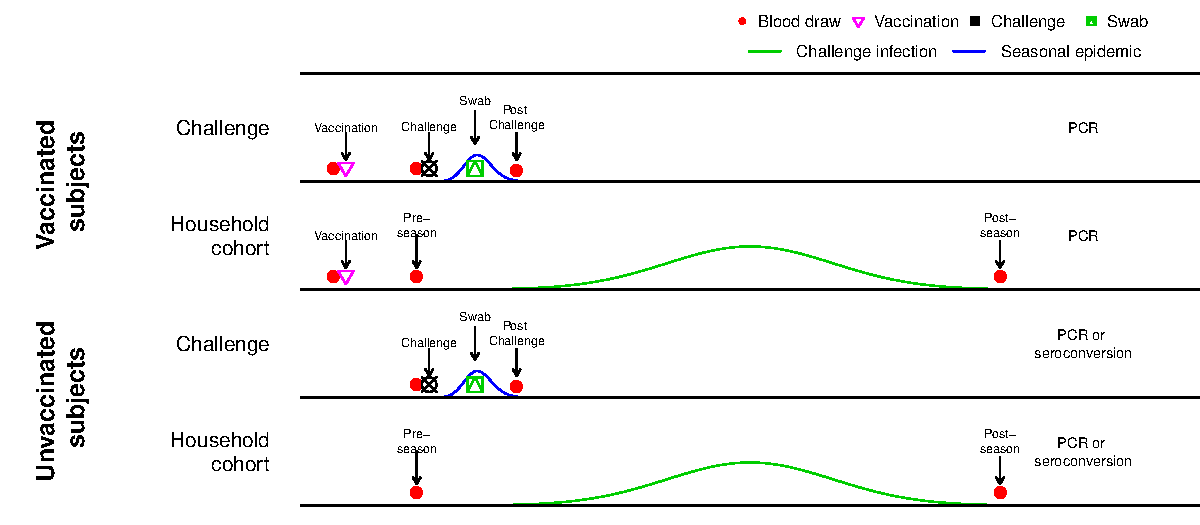
\includegraphics[width=\linewidth]{../fig-studies/fig-studies.pdf}
	\caption{\footnotesize
	Example study designs for the estimation of protective titres.
}
\label{Studies}
\end{figure}


%==============================================================================
\section{Models}

We will discuss all 3 models in the context of a binary outcome $Y$ representing the infection status where 0 --- not infected, 1 --- infected, and a continuous covariate $X$ representing the log-titre measurement. The fitting of all models will be done using the standard maximum likelihood framework. 

All observations with missing values will be removed. All censored titre observation will be handled as follows: below-detectable values will be set to half of the lowest detectable level (lowest detectable level is 10, so the below-detectable values are "imputed" as 5), above-detectable values will be set to the highest dilution used, the other values will be set to the geometric mean of the corresponding interval, e.g. a value of 20 would be shifted to the geometric mean of 20 and 40.


%------------------------------------------------------------------------------
\subsection{Cox proportional hazards}

The Cox PH is a common approach to analysing time-to-event data \cite{George;2014}. It assumes that the subjects being followed up are at risk of an event (e.g., death). This risk can change over time and it is called "hazard" and commonly denoted as $h$. The hazard then is a function of time $t$ and it proportionately changes with covariates.

$$
    h(t) = h_0(t) \ \text{exp}(\beta_XX)
$$

Where $h_0$ is the baseline hazard. In this example, $h_0$ corresponds to the hazard when $X$ (the log-titre) is 0 i.e. at a titre measurement of 1. The coefficient $\beta_X$ corresponds to the change in hazard with a change in $X$. When $X$ increases by 1 (if $X$ is a log2 titre, then this corresponds to a 2-fold titre increase), the hazard changes by $\text{exp}(\beta_X)$, i.e. the hazard is multiplied by a constant.

For the Cox PH regression, the outcome is time-to-event $t$. Infection status $Y$ acts as an indicator of whether the event has occured at the end of the corresponding time period. We will assume that all subjects experience at most one event. In the context of infection this assumption is justified when being infected once grants immunity for the rest of the follow-up period.

Time $t$ is assumed by the model to be time-at-risk of an observable event. For subjects who do not get infected over the follow-up period, $t$ is their total follow-up time and $Y=0$. This represents a right-censored observation, i.e. these subjects "survived" for at least the time they were followed. For subjects who do get infected, $Y=1$ and $t$ is the time it took for them to get infected. The time after infection to end-of-follow-up does not count when we assume that infection grants immunity since the subjects are no longer at risk after infection.

Once the model is fitted, protection $D$ at different values of $X$ can be generated as follows

\begin{gather}
    D(X) = \text{exp}(\hat{\beta}_X X) = \frac{\hat{h}(t)}{\hat{h}_0(t)}
    \label{eq:cox-prot}
\end{gather}

Where $\hat{\beta}_X$ is the estimate of $\beta_X$ and $\hat{h}$ is the estimated hazard.

The quantity in Eq.~\ref{eq:cox-prot} represents the hazard at a given $X$ relative to the baseline hazard (i.e., hazard when $X=0$). If a threshold other than $0$ is desired, the $X$ values can be centered around the desired threshold (e.g., $\text{log}(5)$) prior to fiting the model.


%------------------------------------------------------------------------------
\subsection{Logistic regression}

The logistic model assumes that the probability of outcome follows a logistic curve from 1 (at low covariate values assuming a protective covariate) to 0 (at high covariate values). If there is only one covariate which is the antibody titre measurement, then the model is:

\begin{align*}
    \begin{gathered}
        P(Y=1) = \frac{\text{exp}(\beta_0 + \beta_X X)}{1 + \text{exp}(\beta_0 + \beta_X X)} = \text{logit}^{-1}(\beta_0 + \beta_X X)
    \end{gathered}
\end{align*}

Where $\beta_0$ is the log-odds of infection when $X=0$ and $\beta_X$ is the log-odds ratio of infection of subjects with a given $X$ compared to subjects subjects whose $X$ is 1 unit lower. Note that the linear predictor $L(X)$ is equal to $\beta_0 + \beta_X X$.

Once the model is fitted, estimates of $\beta_0$ ($\hat{\beta}_0$), $\beta_X$ ($\hat{\beta}_X$) are obtained, as well as their variance-covariance matrix which has three terms --- $\text{Var}(\hat{\beta}_0)$, $\text{Var}(\hat{\beta}_X)$ and $\text{Cov}(\hat{\beta}_0, \hat{\beta}_X)$.

One way to generate a protection curve from this model is to subtract the fitted probability $\hat{P}$ from 1

\begin{gather}
    D(X) = 1 - \hat{P}(Y=1)
    \label{eq:lr-prot-abs}
\end{gather}

The quantity in Eq.~\ref{eq:lr-prot-abs} represents the probability of not getting infected (i.e., the probability of being protected) at a given $X$.

The confidence interval for the quantity in Eq.~\ref{eq:lr-prot-abs} can be generated from the interval for $L(X)$ as follows

\begin{gather*}
    \big(\hat{D}(X)_{\text{low}},~\hat{D}(X)_{\text{high}}\big)  =
    \big(
    1 - \text{logit}^{-1}(\hat{L}(X)_{\text{high}}),~
    1 - \text{logit}^{-1}(\hat{L}(X)_{\text{low}})
    \big)                                                       \\
    \big(\hat{L}(X)_{\text{low}},~\hat{L}(X)_{\text{high}}\big)  =
    \big(
    \hat{L}(X) - 1.96 \sqrt{\text{Var}(\hat{L}(X))},~
    \hat{L}(X) + 1.96 \sqrt{\text{Var}(\hat{L}(X))}
    \big)                                                       \\
    \hat{L}(X) = \hat{\beta}_0 + \hat{\beta}_XX \quad
    \text{Var}(\hat{L}(X)) = X^2\text{Var}(\hat{\beta}_X) + \text{Var}(\hat{\beta}_0) + X \text{Cov}(\beta_0, \beta_X)
\end{gather*}

Another way to generate a protection curve from the logistic model is to divide the fitted probability of infection at a given $X$ by the fitted propbability of infection when $X$ is equal to some threshold, e.g. $\text{log}(5)$, to obtain the relative probability of infection and then subtract this quantity from 1

\begin{gather}
    D(X) = 1 - \frac{\hat{P}(Y=1 | X)}{\hat{P}(Y=1 | X = \text{log}(5))}
    \label{eq:lr-prot-rel}
\end{gather}

The quantity in Eq.~\ref{eq:lr-prot-rel} represents the probability of being protected at a given $X$ relative to the probability of protection when $X$ is equal to $\text{log}(5)$.

Note that it is difficult to obtain the confidence interval of the quantity in Eq.~\ref{eq:lr-prot-rel} analytically, so a method such as bootstrapping may be required.
Bootstrapping involves generating random resamples from the data, fitting the model to each one and generating the quantity in Eq.~\ref{eq:lr-prot-rel} at a range of $X$ values for each obtained estimate of $\beta_0$ and $\beta_X$.
After fitting the model to $n$ resamples of the original data, $n$ estimates of protection would be obtained at a range of $X$ values.
The 2.5\% and 97.5\% quantiles of the distribution of protection at any $X$ value formed by the $n$ estimates of protection obtained by bootstrapping can serve as the bounds of the 95\% confidence interval for protection at that $X$ value.


%------------------------------------------------------------------------------
\subsection{Scaled logistic regression}

The scaled logit model is the same as logistic regression except that it estimates the baseline probability of outcome (i.e., the probability at low covariate values assuming a protective covariate) as opposed to assuming that it is equal to 1 \cite{Dunning;2006}. If there is only one covariate which is the antibody titre measurement then the model is

\begin{align*}
    \begin{gathered}
        P(Y=1) = \frac{\lambda}{1 + \text{exp}(\beta_0 + \beta_X X)}
    \end{gathered}
\end{align*}

Note that with the above parameterisation, the $\beta_0$ and $\beta_X$ parameters are negated relative to logistic regression. The new parameter $\lambda$ is the baseline risk, $\text{exp}(\beta_0)$ is the reduction in the baseline risk (protection) at $X=0$, $\beta_X$ is the ratio of protection of subjects with a given $X$ compared to subjects whose $X$ is 1 unit lower.

The baseline risk parameter $\lambda$ is bounded to $[0, 1]$. This may present problems for optimisation. The model can be parameterised as follows to avoid bounded parameters

\begin{gather*}
    P(Y=1) = \frac{\text{exp}(\theta)}{(1 + \text{exp}(\theta))(1 + \text{exp}(\beta_0 + \beta_X X))}
\end{gather*}

Where $\theta$ is baseline log-odds rather than baseline probability.

$$
    \theta = \text{log}\frac{\lambda}{1 - \lambda}
$$

With either parameterisation, the protection is

\begin{gather}
    D(X) = 1 - \frac{\hat{P}(Y=1)}{\hat{\lambda}} = \frac{\text{exp}(\hat{\beta}_0 + \hat{\beta}_X X)}{1 + \text{exp}(\hat{\beta}_0 + \hat{\beta}_X X)}
    \label{eq:sclr-prot}
\end{gather}

The quantity in Eq.~\ref{eq:sclr-prot} represents the reduction in the baseline probablity of infection at a given $X$.


%==============================================================================
\section{Ha Nam application}

This section shows an application of the logistic and the scaled logit models to the H3N2 subset of the data from the Ha Nam cohort which is plotted in Figure \ref{HanamCounts}. The Cox model was not used due to absence of reliable data on disease activity.

\begin{figure}[htp]
	\centering
	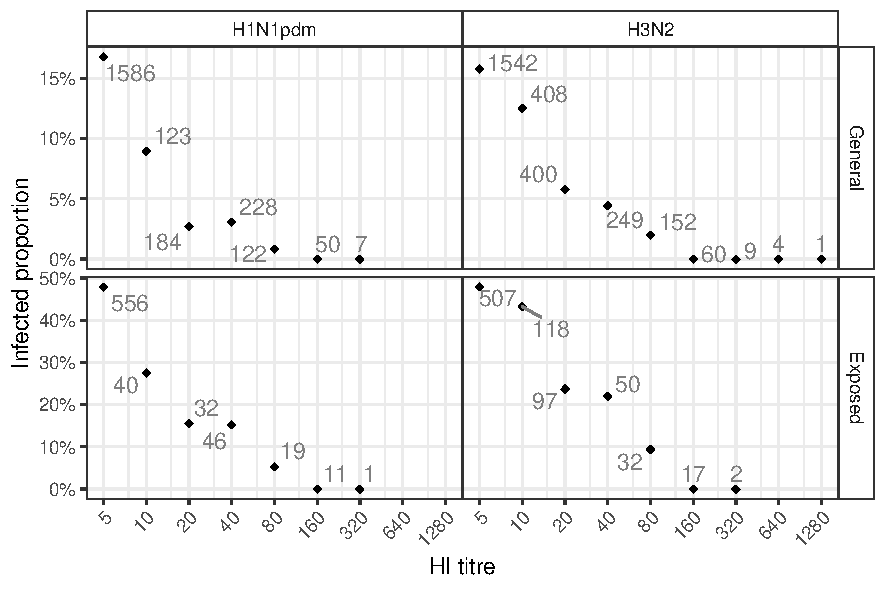
\includegraphics[width=0.9\textwidth]{../data-plot/hanam-hi-summ-light.pdf}
	\caption{
		Ha Nam cohort data. Subjects were grouped by virus and measured HI titre. Numbers next to points are the total number of observations in the corresponding group. The top row is all observations. The bottom row are the observations from households with at least one infection in a given season. The left column is observations for the H1N1pdm virus, the right row --- for H3N2 virus.
	}
	\label{HanamCounts}
\end{figure}


%------------------------------------------------------------------------------
\subsection{Scaled logit fit}

The scaled logit model was fit using the maximum likelihood method. Titre measurement of 5 (below detectable) and 1280 (above detectable) were unchanged, all other observations were moved to the midpoint of the corresponding censored interval on a log scale) The fitted protection curves are in Figure \ref{fig:fit-sclr-prot}.

\begin{figure}[htp]
	\centering
	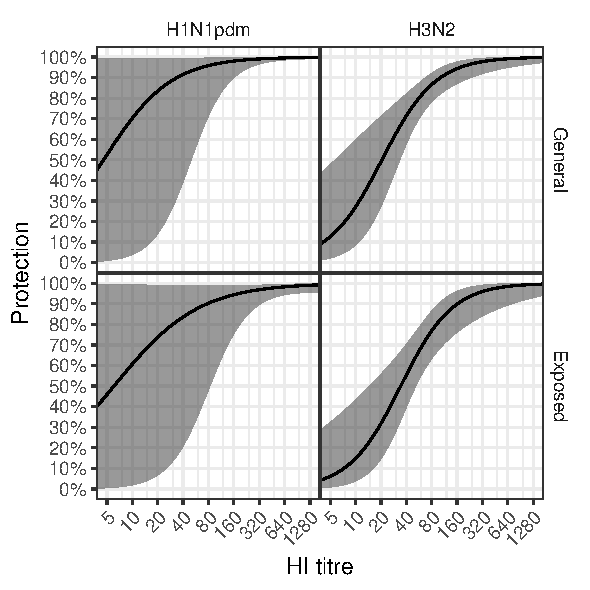
\includegraphics[width=0.8\textwidth]{../fit-sclr-plot/hanam-hi-prot.pdf}
	\caption{
	Fitted protection curves and confidence intervals from the scaled logit fit to Ha Nam data (also shown in Figure \ref{HanamCounts}) using the maximum likelihood method. The solid line is the point estimate. The shaded region is the 95\% confidence interval.
	}
	\label{fig:fit-sclr-prot}
\end{figure}

There is not enough data in the H1N1pdm subset to generate useful estimates. For H3N2 subset, limiting the sample to just those exposed to the virus (at least one household infection in a season) improved the precision of the estimates and shifted curves to the right suggesting that mixing exposed and those potentially not exposed may lead to an overestimate of protection. The general lack of precision in the estimates is likely due to the number of parameters in the model (3 parameters with 1 covariate) and the censored nature of HI titre measurements. In particular, the fact that any titre below 10 is undetectable which means that it is impossible to distinguish between many of the observations (e.g. some subjects with undetectable titres may have had a true titre of 9 while others --- of 2, but both were recorded as 5) and hence it is harder to estimate the baseline probability (as seen in the confidence bounds increasing at small (<10) titres).


%------------------------------------------------------------------------------
\subsection{Comparison to standard logistic fit}

As mentioned before, the standard logistic model is inappropriate due to unsatisfied assumption of baseline of 1. It was fit to the same Ha Nam data using maximum likelihood with no accounting for censored titres (observations of 5 (below detectable) and 1280 (above detectable) were unchanged, all other observations were moved to the midpoint of the corresponding censored interval on a log scale). The fitted infection curve is in Figure \ref{lr-inf}.
-ba
\begin{figure}[htp]
	\centering
	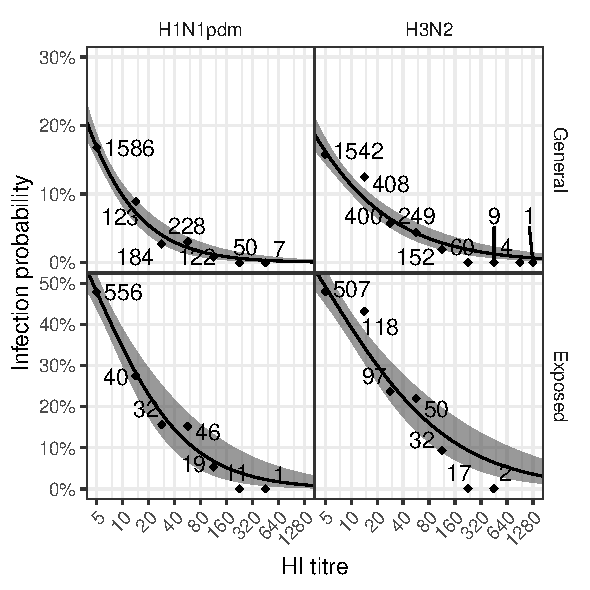
\includegraphics[width=0.8\textwidth]{../fit-logistic-plot/hanam-hi-inf.pdf}
	\caption{
	Fitted infection curves and confidence intervals from the standard logistic model fit to Ha Nam data (also shown in Figure \ref{HanamCounts}) using maximum likelihood with no accounting of censored titres (observations of 5 (below detectable) and 1280 (above detectable) were unchanged, all other observations were moved to the midpoints of the corresponding censored intervals on a log scale). The points are the infected proportions at the corresponding modified titre measurements (i.e. interval midpoints). The solid line is the point estimates. The shaded region is the 95\% confidence interval. The numbers next to the points are the total sample size of the corresponding groups.
	}
	\label{lr-inf}
\end{figure}

%\pagebreak

While the infection curves appear to fit the data well, it is problematic to generate a protection curve from these results. There are two options for the protection curve. One is to use the same procedure as was used in the scaled logit fit --- divide the fitted infection probabilities by the baseline (here assumed to be 1, so the fitted values would not change) and subtract the resulting relative-to-baseline infection probabilities from 1. The protection curves resulting from this procedure are in Figure \ref{lr-prot-abs}.

\begin{figure}[htp]
	\centering
	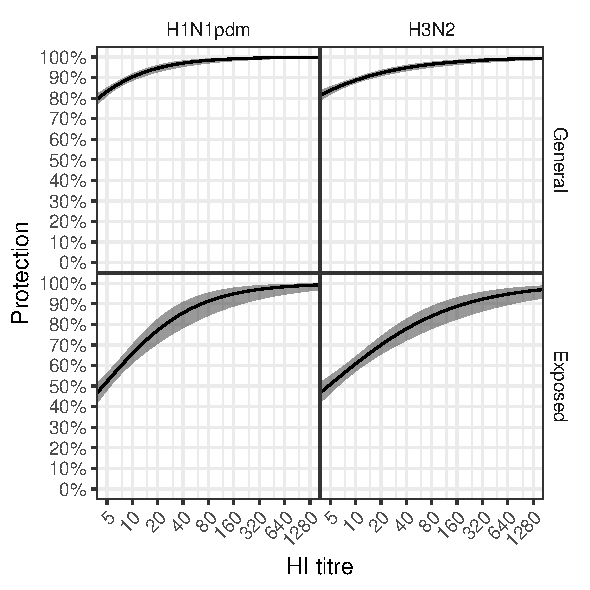
\includegraphics[width=0.8\textwidth]{../fit-logistic-plot/hanam-hi-prot.pdf}
	\caption{
	Fitted protection curves and confidence intervals from the standard logistic model fit to Ha Nam data (also shown in Figure \ref{HanamCounts}) using maximum likelihood with no accounting of censored titres (observations of 5 (below detectable) and 1280 (above detectable) were unchanged, all other observations were moved to the midpoints of the corresponding censored intervals on a log scale). The solid line is the point estimates. The shaded region is the 95\% confidence interval.
	}
	\label{lr-prot-abs}
\end{figure}

The other option for generating a protection curve is to calculate the fitted probability of infection at a give titre and divide that by the fitted probability of infection at the titre of 5 (or any other) thereby generating a curve that shows relative-to-5 infection probabilities (as opposed to relative-to-baseline). The variance of this quantity may be estimated by using the bootstrap method. Subtracting these relative-to-5 infection probabilities from 1 generates curves shown in Figure \ref{lr-prot-rel}.

%\pagebreak

\begin{figure}[htp]
	\centering
	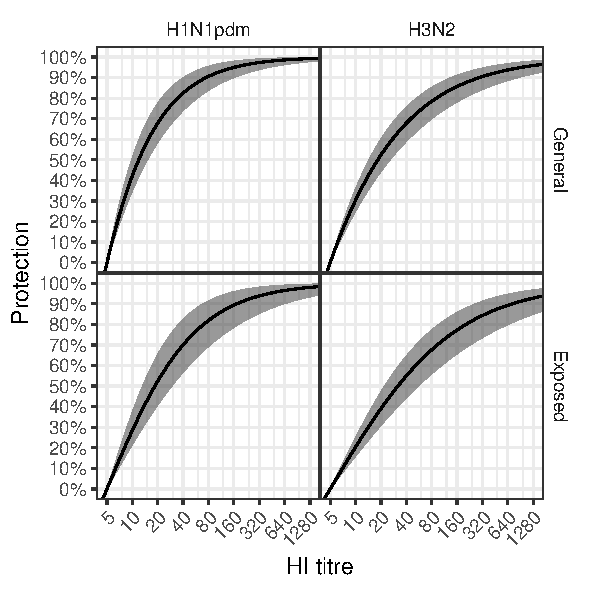
\includegraphics[width=0.8\textwidth]{../fit-logistic-boot-plot/hanam-hi-prot-rel.pdf}
	\caption{
	Fitted relative-to-5 protection curves and confidence intervals from the standard logistic model fit to Ha Nam data (also shown in Figure \ref{HanamCounts}) using maximum likelihood with no accounting of censored titres (observations of 5 (below detectable) and 1280 (above detectable) were unchanged, all other observations were moved to the midpoints of the corresponding censored intervals on a log scale). Solid lines are the point estimates, with shaded regions the 95\% confidence interval. The bounds for the confidence interval were obtained by using the bootstrap method (10,000 samples).
	}
	\label{lr-prot-rel}
\end{figure}

While the relative-to-5 protection curves (Figure \ref{lr-prot-rel}) appear more plausible than the relative-to-baseline protection curves (Figure \ref{lr-prot-abs}), both result from fitting a model with an unsatisfied assumption and neither method of generating protection curves from logistic regression model reliably produce accurate results.

The relative-to-5 curve (Figure \ref{lr-prot-rel}) presents an additional problem. The curve shows how much ``better'' different titres are at protecting against infection than the titre of 5. 
There is nothing inherently special about this threshold of 5. Its choice is based on the lower dilution of 10. Pre-treatment of the sera necessitates dilution, so the lower bound can never be 1, but could be something more than 1 such as <5.  Nevertheless, the curves may look substantially different if a different threshold (e.g. 10 or 1) is chosen.


%==============================================================================
\section{Kiddyvax application}

The data for this study includes post-vaccination HI titres of subjects who were followed for up to one year for flu infection. The infection status was determined by PCR which was done for everyone who experienced symptoms. This data is shown in Figure \ref{fig:kiddyvax-main-titre}.

\begin{figure}[htp]
	\centering
	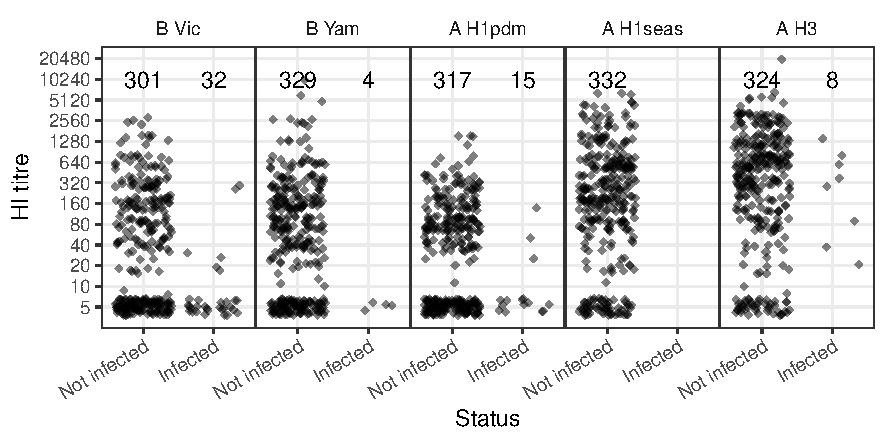
\includegraphics[width=1\textwidth]{../data-plot/kiddyvax-main-titre.pdf}
	\caption{
	Kiddyvax study data. Post-vaccination titres are shown for those who got infected (PCR-confirmed symptomatic infection) over the course of the study and those who did not. Panels correspond to the five tested viruses.
	}
	\label{fig:kiddyvax-main-titre}
\end{figure}

Analyses were done on the data for B Vic and A(H1pdm) viruses in the same way as for the Ha Nam data with the addition of the Cox proportional hazards model.


%------------------------------------------------------------------------------
\subsection{Scaled logit fit}

The same scaled logit model was fit in the same way as for the Ha Nam data. The protection curves are in Figure \ref{fig:kiddyvaxmain-sclr-prot}. The model fails to produce useful estimates due to there being very few infections in the sample.

\begin{figure}[htp]
	\centering
	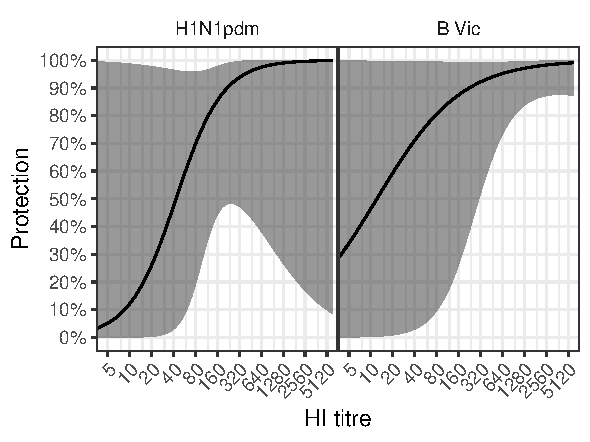
\includegraphics[width=0.8\textwidth]{../fit-sclr-plot/kiddyvaxmain-prot.pdf}
	\caption{
	Fitted protection curves and confidence intervals from the scaled logit fit to H1N1pdm and H3N2 subsets of Kiddyvax data (also shown in Figure \ref{fig:kiddyvax-main-titre}) using the maximum likelihood method. The solid line is the point estimate. The shaded region is the 95\% confidence interval.
	}
	\label{fig:kiddyvaxmain-sclr-prot}
\end{figure}


%------------------------------------------------------------------------------
\subsection{Standard logistic fit}

The relative protection curves are in Figure \ref{fig:kiddyvaxmain-prot-rel-lr-boot}. The same considerations regarding the unjustified assumption of baseline risk of 1 apply here as they did with Ha Nam (Figure \ref{fig:kiddyvax-main-titre} shows many uninfected subjects with undetectable titres).

\begin{figure}[htp]
	\centering
	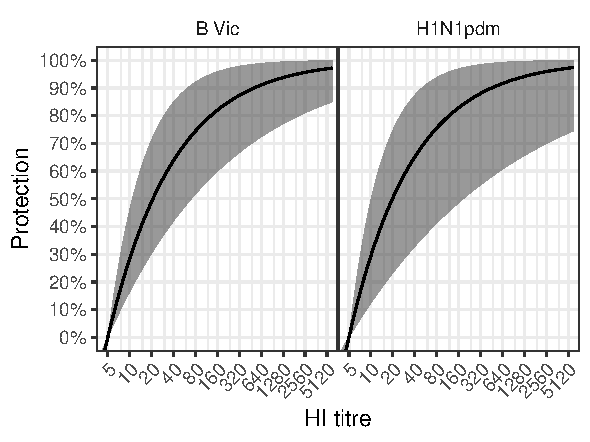
\includegraphics[width=0.8\textwidth]{../fit-logistic-boot-plot/kiddyvaxmain-prot-rel.pdf}
	\caption{
	Fitted relative-to-5 protection curves and confidence intervals from the standard logistic model fit to H1N1pdm and H3N2 subsets of kiddyvax data (shown in Figure \ref{fig:kiddyvax-main-titre}) using maximum likelihood with no accounting of censored titres (observations of 5 (below detectable) were unchanged, all other observations were moved to the midpoints of the corresponding censored intervals on a log scale). The solid line is the point estimates. The shaded region is the 95\% confidence interval. The bounds for the confidence interval were obtained by using the bootstrap method (10,000 samples).
	}
	\label{fig:kiddyvaxmain-prot-rel-lr-boot}
\end{figure}


%------------------------------------------------------------------------------
\subsection{Cox proportional hazards fit}

For infected individuals, the time at risk was taken to be the time from start of follow-up to infection. For those who did not get infected the time at risk was take to be the time from start of follow-up to end of follow-up.

The model was

\begin{align*}
\begin{gathered}
h(t) = h_0\text{exp}(\beta_T X_{\text{logtitre}})
\end{gathered}
\end{align*}

where $h$ is the hazard function and $X_{\text{logtitre}}$ is the post-vaccination titre measurement on the log scale. The resulting protection curves (relative to the titre of 5) are in Figure \ref{fig:kiddyvaxmain-cox}. Although the point estimates are similar to those recovered from the model; however standard errors are inflated.

\begin{figure}[htp]
	\centering
	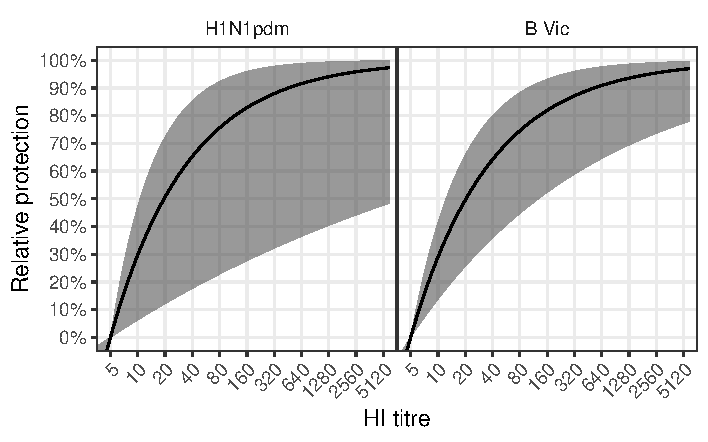
\includegraphics[width=0.8\textwidth]{../fit-cox-plot/kiddyvaxmain.pdf}
	\caption{
	Fitted relative-to-5 protection curves and confidence intervals from the Cox proportional hazards model fit to H1N1pdm and H3N2 subsets of kiddyvax data (shown in Figure \ref{fig:kiddyvax-main-titre}) with no accounting of censored titres (observations of 5 (below detectable) were unchanged, all other observations were moved to the midpoints of the corresponding censored intervals on a log scale). The solid line is the point estimates. The shaded region is the 95\% confidence interval.
	}
	\label{fig:kiddyvaxmain-cox}
\end{figure}


%==============================================================================
\section{Conclusion}

\begin{table}[htp]
\centering
\caption{Summary of the three considered models in terms of their application to antibody data}
\begin{tabular}{cp{25em}}
\toprule
Model & Potential problem \\
\midrule
Cox PH & Biased if follow-up time is not proportional to time at risk for everyone in the sample \\
Logistic & Biased if low antibody titres do not guarantee immunity \\
Scaled logit & Requires a large sample size. \\
\bottomrule
\end{tabular}
\end{table}

In this paper we have explored three different models for estimating protective antibody titres using data from influenza vaccine and infection studies.  We have shown that in the presence of good time-to-event data where every subject's follow-up time is at least proportional to their time at risk, the Cox model will likely perform best out the three models explored due to it having the least number of parameters allowing for more precise estimates. Absent such data, logistic regression may be appropriate if the assumption of everyone being infected at low antibody titres can be justified. If this assumption cannot be justified, which is probably the case for influenza studies, the scaled logit model can be applied but the sample needs to be fairly large (>500) in order to obtain useful estimates.


\pagebreak
%=============================================================================
\bibliography{bibliography}
All code is in github.com/khvorov45/model-comparison

\end{document}
